%======================================================================
\chapter{Introduction}
%======================================================================

%----------------------------------------------------------------------
\section{Background}
%----------------------------------------------------------------------
Japan has long been one of the most popular tourist destinations in Asia. Before the spread of Covid-19, the number of foreign visitors to Japan gradually increased. According to Japan National Tourism Organization (JNTO) statistics, the number of foreign visitors more than quadrupled between 2012 (8.36 million) and 2019 (31.9 million) that shown in Figure~\ref{fig1}. As a result, the Japan National Tourism Organization has been working hard over the years to assist foreign visitors to have a better experience in Japan. Considering that Japan is a relatively disaster-prone country, disaster prevention for foreign visitors during their stay in Japan has been an issue of great concern to the Japan National Tourism Organization.

%%%%%%%%%%%%%%%%%%%%%
%\iffalse
\begin{figure*}[h]
  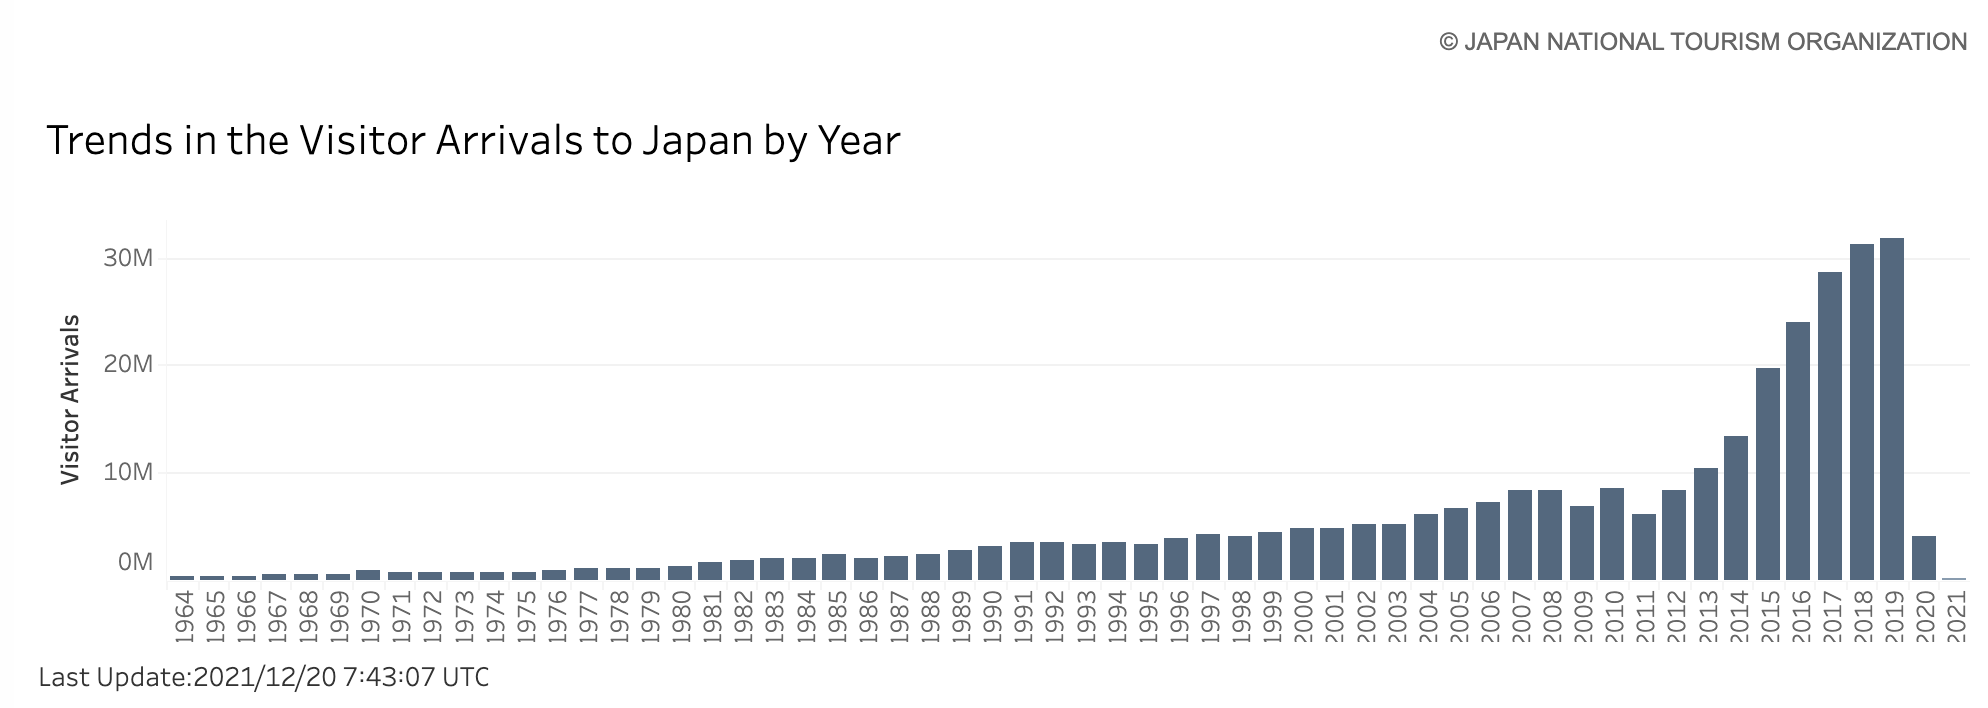
\includegraphics[width=\linewidth]{Figure/Figure1.png}
  \centering
  \caption[Foreign visitors number in Japan by year.]{Foreign visitors number in Japan by year.\protect\footnotemark }
  \label{fig1}
\end{figure*}
\footnotetext{\url{https://statistics.jnto.go.jp/en/graph/\#graph--inbound--travelers--transition}}
%\fi
Combined with the previous studies which will review in Chapter~\ref{c2}, it is clear that providing information in foreign visitors' native language as well as evacuation assistance is really important during evacuation. Also, there is a need to provide sufficient places for foreign visitors to recharge to ensure that they can contact their family/friends and gather the necessary disaster information from social media/networks survey~\cite{ref50}. Kawasaki (2012)~\cite{ref48} also verified the problems that occurred during evacuation caused by language barriers. Sakurai 2020~\cite{ref46} also mentioned that the Government, as a national agency, should work with communicators to deliver as much information as possible in the event of a disaster and that these guidelines should be posted on social media. The information needs to be multilingual, and the symbols need to be more circulated to help foreign visitors who do not understand Japanese well. Kawasaki (2018)~\cite{ref47} also indicated that foreigners with strong Japanese language skills have similar information-gathering behavior to Japan, but that foreigners who do not know much about Japan rarely use media that focus on the Japanese language. This group also encounters difficulties in evacuation due to language limitations, as they can only rely on a small amount of information that can be provided in their native language for evacuation information search.

Precisely for this reason, the Japan Tourism Agency has constantly been concerned with issues of security and safety in the tourism industry. So, under the supervision of the Japan Tourism Agency, R.C. Solutions, Inc. developed a free application called Safety Tips. Safety Tips can notify foreign visitors of earthquake early warnings, tsunami warnings, eruption alerts, special warnings, heatstroke information, national protection information, evacuation advisories, and other disasters that occurred in Japan. Figure~\ref{fig3} shows the Safety Tips interface.  Based on previous research, this application can largely solve the problems that foreign visitors encounter in the evacuation process due to the language barrier, as Safety Tips can provide a variety of purposes for foreign visitors to Japan. It is available in 14 languages (15 languages), including Japanese, English, Chinese (traditional and simplified), Korean, Spanish, Portuguese, Vietnamese, Thai, Indonesian, Tagalog, Nepali, Khmer, Burmese, and Mongolian (as shown in Figure~\ref{fig4}). Safety Tips is an important part of this study. In order to make Safety Tips better for foreign visitors to utilize during the evacuation, this study will compare the difference in perceptions on Safety Tips among respondents of various nationalities, as well as the differences in perceptions on Safety Tips among people from various upbringing backgrounds. By understanding these differences and how personal backgrounds affect people's perception of Safety Tips, we can use the results to make recommendations that will help Safety Tips develop.






%%%%%%%%%%%%%%%%%%%%%%%%%%%%%%%%
%\iffalse
\begin{figure*}[h]
  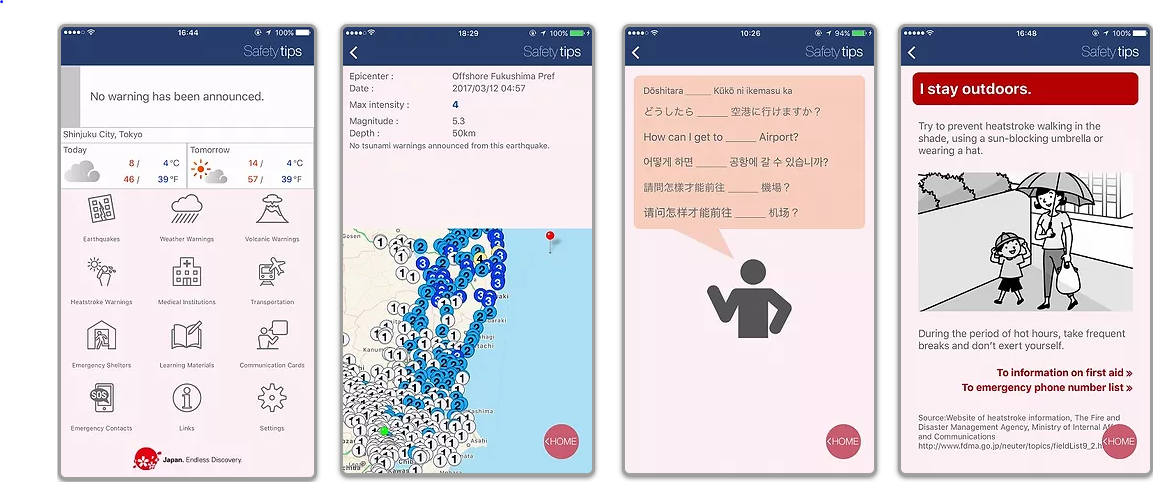
\includegraphics[width=\linewidth]{Figure/Figure3.png}
  \centering
  \caption[Safety Tips' interface]{Safety Tips' interface.\protect\footnotemark }
  \label{fig3}
\end{figure*}
\footnotetext{\url{https://www.rcsc.co.jp/safety}}

\begin{figure*}[h]
  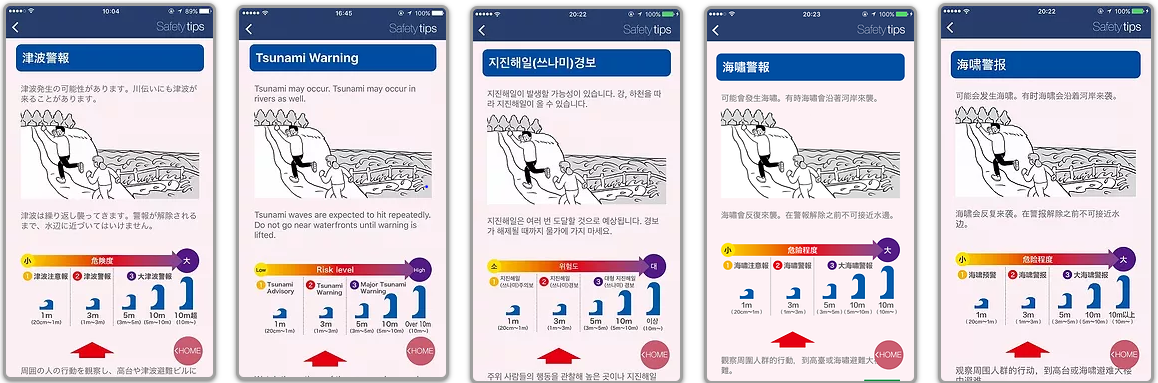
\includegraphics[width=\linewidth]{Figure/Figure4.png}
  \centering
  \caption[Multilingual Notifications for Safety Tips]{Multilingual Notifications for Safety Tips\protect\footnotemark }
  \label{fig4}
\end{figure*}
\footnotetext{\url{https://www.rcsc.co.jp/safety}}
%\fi

\section{Research Problem Identification}
Based on the above, we can understand that foreign visitors will face numerous challenges when a disaster strikes while visiting. Because earthquakes and other natural disasters are relatively common in Japan, Japanese children learn about evacuation at a young age and participate in numerous evacuation/evacuation drills and exercises. However, there would be many differences between Japanese and foreign visitors. For example, for foreign visitors, it is unknown whether they have previously experienced disasters, whether they learned about evacuation as children, or whether they have participated in earthquake simulation drills. As a result, they would behave differently with the Japanese during the evacuation. 

Therefore, it is important to explore the behavioral differences between foreign visitors and Japanese. In many cases, it is not very helpful to set up disaster prevention programs only according to the behavior of Japanese people. Only when we clearly understand the differences in behavior between Japanese and foreign visitors, and then think about how to help them according to the behavior of foreign visitors, can we better build disaster prevention programs. In order to achieve this, the results of the selection of response actions were analyzed in this study to explore evacuation behavior preferred by foreign visitors, as well as the differences between Japanese and foreign visitors.

On the other hand, whether the respondents' perception ons Safety Tips is influenced by some demographic information such as country, age, gender, and their past experiences is also a problem that this study wants to explore. It is hoped that this study will help to find out the reasons for the different perceptions of Safety Tips so that Safety Tips can be better developed.

\section{Research Goal and Objective}
The goal of this study is to clarify the information-seeking and evacuation behavior of foreign visitors to Japan, as well as their perception of Safety Tips. This study has three main research objectives. 

\begin{itemize}
\item Objective 1: To understand foreign visitors' perception on Safety Tips.
\item Objective 2: To explore how respondents' perceptions on Safety Tips are influenced by their characteristics.
\item Objective 3: To explore response behaviors of information seeking and evacuation.
\end{itemize}

Finally, based on the findings of the research, provide improvement suggestions to Safety Tips.


\section{Thesis Structure} 

This thesis begins with the first chapter, introduction, which explains the study's background, research questions, objectives and goals, and thesis structure. The introduction chapter's purpose is to provide background for the entire study and to help the reader in understanding the research topic. Then, the second chapter of the thesis focuses on the literature review. Considering that in this study, it is necessary to make the basic hypothesizes of Structural Equation Modeling based on prior research, Chapter~\ref{c2} reviews some relevant studies in the field of evacuation research and provide an idea for the basic hypothesizes of relationships between factors like demographic information, educational background, past disaster experience, and disaster training experience. The information of the survey and data used in this study are presented in Chapter~\ref{c3}. Because the data in this study is extensive and complex, we intend to provide a more complete description in Chapter~\ref{c3} to help the reader understand it better. 

To make Safety Tips more useful to foreign visitors, Chapter~\ref{c4} aims to achieve objective 1, which is to understand respondents' perceptions on the use of Safety Tips. Then, Chapter~\ref{c5} is to achieve objective 2, which is to explore whether those characteristics will influence respondents'  perceptions on Safety Tips or not. The characteristics include nationality, age, travel experience, disaster prevention education level, language ability, disaster experience, training experience, disaster prevention consciousness. These are discussed in depth in Chapter~\ref{c5}. Chapter~\ref{c6} is to achieve objective 3, which explores the response actions during evacuation. There have two subsections for Chapter 4 to Chapter 6, which are methodology, results, and discussions. The methodology includes the introduction and academic explanation of each method used to achieve each of the research objectives. The results and analysis show and analyze the results one by one since this research is based on the analysis of data to clarify foreign visitors' behaviors and perceptions, then to make suggestions of Safety Tips. The final chapter, Chapter~\ref{c7}, is the conclusion section. This chapter contains a summary conclusion of the whole study, some suggestions based on the results to help Safety Tips for better development, and the limitations in this study.

%%%%%%%%%%%%%%%%%%%%%%%%%%%%
%\iffalse

%\fi


